\chapter{T-Dualität, D-Branen und Eichtheorie}

\lectureoverview{Die T-Dualität beginnt als exakte Äquivalenz zwischen geschlossenen
Strings auf Kreisen mit den Radien (R) und \(\alpha'/R\). Impuls und Windungszahl
tauschen ihre Rollen, ebenso die Weltblatt-Ableitungen \(\partial_\tau Y\) und
\(\partial_\sigma Y\) sowie die Raumzeitvektoren, die aus \(G_{\mu 5}\) und \(B_{\mu 5}\) hervorgehen. Wird dieselbe Operation auf einen offenen String angewandt, wird aus einer Neumann-Randbedingung eine Dirichlet-Randbedingung.
Der Endpunkt muss dann auf einer dynamischen D-Brane liegen. Offene Strings, die auf eine einzelne Brane beschränkt sind, ergeben bei niedrigen Energien eine abelsche Eichtheorie; Strings, die eine Gruppe von Branen verbinden, tragen zwei Endpunktindizes und ergeben eine nichtabelsche Eichtheorie. Ein D-String, der auf einer D3-Brane endet, liefert den entsprechenden magnetischen Monopol.}

\section{Warum kehren wir zur T-Dualität zurück?}

Wir sind der T-Dualität bereits begegnet, kommen aber aus gutem Grund auf sie zurück. Sie war einer der Hinweise darauf, dass die Stringtheorie weit mehr als perturbative Strings umfasst. Als man die Konsequenzen für offene Strings verstanden hatte, führte dies zu D-Branen; diese wurden ihrerseits zu einem Mittel, Quantenfeldtheorien zu konstruieren und zu untersuchen. Ziel dieser Vorlesung ist es daher nicht, lediglich das Schlagwort zu wiederholen, ein kleiner Kreis sei einem großen Kreis äquivalent. Wir werden die Argumentation sorgfältig genug rekonstruieren, um zu erkennen, wie dieses Schlagwort die Theorie dazu zwingt, neue physikalische Objekte zu enthalten.

Die einfachste Ausgangslage ist die toroidale Kompaktifizierung. Ein eindimensionaler Torus ist ein Kreis. Ein zweidimensionaler Torus lässt sich als Parallelogramm darstellen, dessen gegenüberliegende Seiten identifiziert werden, und ein dreidimensionaler Torus als Parallelepiped, dessen gegenüberliegende Flächen identifiziert werden. Dieselbe Konstruktion lässt sich auf höhere Dimensionen übertragen. Wir betrachten nur eine kompakte räumliche Koordinate, bezeichnet mit \(Y\), und eine repräsentative nichtkompakte Koordinate, bezeichnet mit \(X\). Die Zeit ist vorhanden, wird in den Tafelzeichnungen jedoch nicht dargestellt.

Wir wählen die übliche Konvention
\begin{equation}
  Y\sim Y+2\pi R,
  \label{eq:l10-circle-identification}
\end{equation}
sodass \(R\) der Radius und \(2\pi R\) der Umfang ist. In der Vorlesung wird die kompakte Größe oft einfach \(r\) genannt; dabei werden Faktoren von \(2\pi\) und \(\alpha'\) weggelassen. Bei den Herleitungen behalten wir die üblichen Faktoren bei und geben die Einheiten der Vorlesung an, wenn sie nützlich sind.

In der ersten Hälfte der Diskussion betrachten wir geschlossene, orientierte Strings. Eine Orientierung ist ein intrinsischer Pfeil, der entlang des Strings eingezeichnet wird. Würde man überall alle Pfeile umkehren, änderte sich kein Experiment; entscheidend ist die relative Orientierung zweier Strings. Beim Aufspalten und Vereinigen müssen die Pfeile stetig zusammenpassen. Das ist der erste Hinweis darauf, dass eine vorzeichenbehaftete Erhaltungsgröße auftreten wird.

\begin{figure}[H]
  \centering
  \includegraphics[width=0.72\textwidth]{lecture_10_figure_01.png}
  \caption{Zwei geschlossene Strings mit ihren relativen Orientierungen, wie an der Tafel eingezeichnet. Die Orientierung muss beim Aufspalten und Vereinigen stetig bleiben.}
  \lectureframe{00:05:40}
  \label{fig:l10-oriented-closed-strings}
\end{figure}

\begin{classroomqa}
\audiencequestion{Ist der String bereits einmal um die kompakte Richtung herumgelaufen, wenn die Weltblattkoordinate von \(\sigma=0\) bis \(2\pi\) reicht? \lecturetimestamp{00:08:42}}
\lecturerresponse{Nein. Die Koordinate \(\sigma\) bezeichnet Punkte entlang des Strings; sie bezeichnet keine Positionen im kompakten Raum. Jeder geschlossene String hat einen periodischen Parameter \(\sigma\), unabhängig davon, ob er gewunden ist oder nicht. Die Analogie mit einem Gummiband ist hilfreich: Man kann die Moleküle entlang eines Gummibands nummerieren, auch wenn es um nichts herumgewickelt ist. Die Windung ist eine Eigenschaft der Abbildung \(Y(\tau,\sigma)\), nicht des Parameters \(\sigma\) allein.}
\end{classroomqa}

\begin{classroomqa}
\audiencequestion{Muss die kompakte Größe auch für jeden Wert der großen Koordinate \(X\) gleich sein? \lecturetimestamp{00:10:00}}
\lecturerresponse{Nicht bei einer allgemeinen dynamischen Kompaktifizierung. Wir beginnen mit einem festen Kreis, weil dieser den übersichtlichsten Hintergrund bildet. Später wird die Komponente \(G_{55}\) zu einem Skalarfeld, dessen Wert die lokale Größe der fünften Richtung angibt; diese Größe kann sich also über der gewöhnlichen Raumzeit ändern.}
\end{classroomqa}

\section{Die Windungszahl bleibt auch beim Wiederverbinden von Strings erhalten}

Ein ungewickelter String kann sich durch die kompakte Richtung bewegen, ohne sie zu umschlingen. Ein gewundener String ist anders: Wenn \(\sigma\) den geschlossenen String einmal durchläuft, schreitet die Einbettung \(Y(\tau,\sigma)\) um eine oder mehrere Perioden des kompakten Kreises fort. Da der String orientiert ist, hat diese Verschiebung ein Vorzeichen. Ein String kann in positiver oder negativer Richtung gewunden sein.

Am deutlichsten wird das Erhaltungsgesetz anhand der Vereinigungsbilder. Betrachten wir einen String mit der Windungszahl \(+1\) und einen zweiten mit der Windungszahl \(-1\). Ihre zueinander passenden Segmente können sich wiederverbinden. Die resultierende Konfiguration hat eine Windungssumme von null und lässt sich zu einem ungewickelten String verformen. Die Zeichnung an der Tafel stellt genau diese Wiederverbindung entgegengesetzter Orientierungen dar.

\begin{figure}[H]
  \centering
  \includegraphics[width=0.72\textwidth]{lecture_10_figure_02.png}
  \medskip

  \begin{tikzpicture}[x=1cm,y=1cm,>=Latex]
    \draw[thick] (-4.0,0.3) circle (0.65);
    \draw[->,thick] (-4.55,0.58) arc (150:-145:0.65);
    \node at (-4.0,-0.65) {$w=+1$};
    \draw[thick] (-2.0,0.3) circle (0.65);
    \draw[<-,thick] (-2.55,0.58) arc (150:-145:0.65);
    \node at (-2.0,-0.65) {$w=-1$};
    \node at (-3.0,0.3) {$+$};
    \draw[->,thick] (-1.0,0.3) -- (0.3,0.3);
    \draw[thick] (1.4,0.3) ellipse (0.95 and 0.55);
    \node at (1.4,-0.65) {$w_{\rm total}=0$};
  \end{tikzpicture}
  \caption{Entgegengesetzte Windungen verbinden sich wieder zu einer Konfiguration mit Windungssumme null. Die untere Zeichnung rekonstruiert den Vorgang an der Tafel, sie zeigt keinen zweiten dynamischen Prozess.}
  \lectureframe{00:13:20}
  \label{fig:l10-opposite-winding}
\end{figure}

Wiederholen wir nun das Experiment mit zwei gleich orientierten Strings. Sie können sich vereinigen, aber nicht abwickeln. Das Ergebnis trägt die doppelte Windungszahl jedes der beiden eingehenden Strings. Die Zahl der zusammenhängenden Strings hat sich geändert, die Gesamtwindungszahl nicht.

\begin{figure}[H]
  \centering
  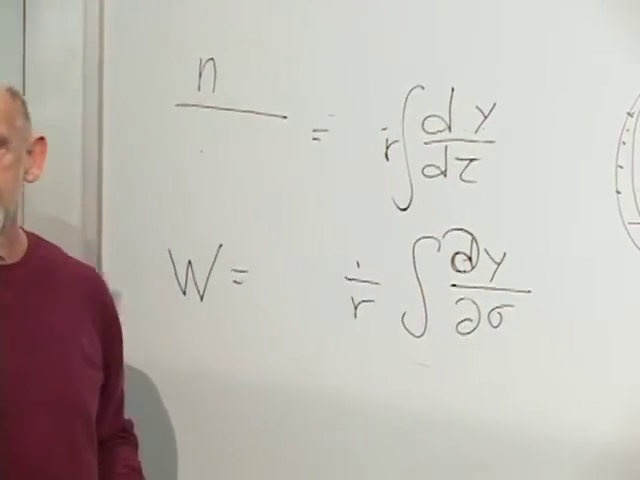
\includegraphics[width=0.72\textwidth]{lecture_10_figure_03.png}
  \medskip

  \begin{tikzpicture}[x=1cm,y=1cm,>=Latex]
    \draw[thick] (-4.0,0.3) circle (0.65);
    \draw[->,thick] (-4.55,0.58) arc (150:-145:0.65);
    \node at (-4.0,-0.65) {$w=+1$};
    \draw[thick] (-2.0,0.3) circle (0.65);
    \draw[->,thick] (-2.55,0.58) arc (150:-145:0.65);
    \node at (-2.0,-0.65) {$w=+1$};
    \node at (-3.0,0.3) {$+$};
    \draw[->,thick] (-1.0,0.3) -- (0.3,0.3);
    \draw[thick] (1.45,0.3) circle (0.78);
    \draw[thick] (1.45,0.3) circle (0.52);
    \draw[->,thick] (0.81,0.74) arc (145:-145:0.78);
    \node at (1.45,-0.78) {$w=+2$};
  \end{tikzpicture}
  \caption{Gleichsinnige Windungen können sich zu einem doppelt gewundenen String verbinden. Die Zusammenhangsstruktur ändert sich, während die Gesamtwindungszahl zwei bleibt.}
  \lectureframe{00:16:40}
  \label{fig:l10-same-winding}
\end{figure}

Diese Unterscheidung bleibt bei jedem erlaubten Prozess bestehen. Eine Gesamtwindungszahl von hundert kann von einem hundertfach gewundenen String, von zwei jeweils fünfzigfach gewundenen Strings oder von hundert einfach gewundenen Strings getragen werden. Strings können sich aufspalten und zu den hier beschriebenen Konfigurationen vereinigen, doch die vorzeichenbehaftete Summe bleibt hundert. Wir bezeichnen sie mit \(w\in\mathbb Z\).

\section{Impulsmoden und Windungsmoden}

Die Erhaltung allein ergibt noch keine Dualität. Als Nächstes vergleichen wir die Energien. Ein Zustand mit Bewegung um den kompakten Kreis hat einen quantisierten Impuls
\begin{equation}
  p_Y=\frac{n}{R},
  \qquad n\in\mathbb Z.
  \label{eq:l10-compact-momentum}
\end{equation}
Wenn die übrigen Massenbeiträge des Zustands vernachlässigt werden können, trägt die Bewegung in kompakter Richtung \(E_{\rm mom}=|n|/R\) bei. Positive und negative Werte von \(n\) bezeichnen entgegengesetzte Bewegungsrichtungen, während die Energie positiv ist.

\begin{figure}[H]
  \centering
  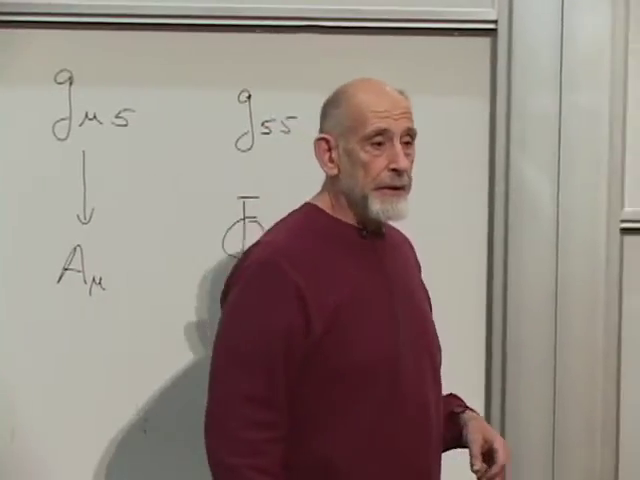
\includegraphics[width=0.72\textwidth]{lecture_10_figure_04.png}
  \caption{Die Quantenzahl des kompakten Impulses an der Tafel. In der Vorlesung wird der Impuls schematisch als Integral der kompakten Geschwindigkeit geschrieben.}
  \lectureframe{00:21:30}
  \label{fig:l10-compact-momentum-board}
\end{figure}

Ein String mit \(|w|\) Windungen hat die Länge \(2\pi |w|R\). Bei einer fundamentalen Stringspannung von
\begin{equation}
  T_{\rm F}=\frac{1}{2\pi\alpha'},
\end{equation}
beträgt seine Windungsenergie
\begin{equation}
  E_{\rm wind}=T_{\rm F}(2\pi |w|R)
  =\frac{|w|R}{\alpha'}.
  \label{eq:l10-winding-energy}
\end{equation}
In den Einheiten der Vorlesung, \(\alpha'=1\), ist dies einfach \(E_{\rm wind}=|w|R\).

Die beiden Türme verhalten sich bei einer Änderung des Radius entgegengesetzt. Für \(R\gg
\sqrt{\alpha'}\) liegen die Impulsniveaus dicht beieinander und die Windungsniveaus weit auseinander. Für \(R\ll\sqrt{\alpha'}\) liegen die Impulsniveaus weit auseinander und die Windungsniveaus dicht beieinander.

\begin{figure}[H]
  \centering
  \begin{minipage}[t]{0.48\textwidth}
    \centering
    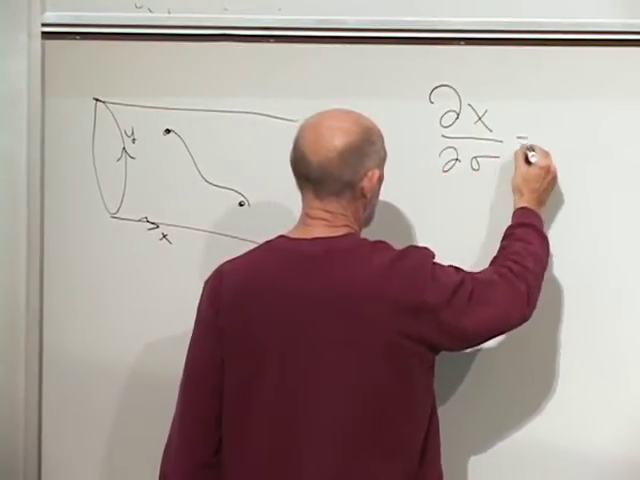
\includegraphics[width=\linewidth]{lecture_10_figure_05.png}
    \par\smallskip
    \textit{Großer kompakter Radius.}
  \end{minipage}\hfill
  \begin{minipage}[t]{0.48\textwidth}
    \centering
    \includegraphics[width=\linewidth]{lecture_10_figure_06.png}
    \par\smallskip
    \textit{Kleiner kompakter Radius.}
  \end{minipage}
  \caption{Die beiden Spektralvergleiche an der Tafel. Bei der Inversion des Radius tauschen die spärlich und dicht besetzten Türme ihre Rollen.}
  \lectureframe{00:25:30--00:26:00}
  \label{fig:l10-dual-spectra-board}
\end{figure}

Das übersichtliche Schema lautet
\begin{figure}[H]
  \centering
  \begin{adjustbox}{max width=\linewidth}
  \begin{tikzpicture}[x=1cm,y=0.74cm,>=Latex]
    \node[font=\bfseries] at (-3.6,6.2) {$R\gg\sqrt{\alpha'}$};
    \draw[->] (-5.1,0) -- (-5.1,5.5) node[above] {$E$};
    \foreach \y in {0.4,1.0,1.6,2.2,2.8,3.4,4.0,4.6}
      \draw (-5.35,\y)--(-4.85,\y);
    \node[align=center] at (-4.25,5.15) {momentum\\dense};
    \draw[->] (-2.2,0) -- (-2.2,5.5) node[above] {$E$};
    \foreach \y in {0.4,2.4,4.4}
      \draw (-2.45,\y)--(-1.95,\y);
    \node[align=center] at (-1.35,5.15) {winding\\sparse};

    \node[font=\bfseries] at (3.6,6.2) {$R\ll\sqrt{\alpha'}$};
    \draw[->] (2.2,0) -- (2.2,5.5) node[above] {$E$};
    \foreach \y in {0.4,2.4,4.4}
      \draw (1.95,\y)--(2.45,\y);
    \node[align=center] at (3.05,5.15) {momentum\\sparse};
    \draw[->] (5.1,0) -- (5.1,5.5) node[above] {$E$};
    \foreach \y in {0.4,1.0,1.6,2.2,2.8,3.4,4.0,4.6}
      \draw (4.85,\y)--(5.35,\y);
    \node[align=center] at (5.95,5.15) {winding\\dense};
  \end{tikzpicture}
  \end{adjustbox}
  \caption{Rekonstruktion des Arguments anhand der Niveauabstände. Das vollständige Stringspektrum bleibt unverändert, wenn Impuls und Windung gemeinsam mit \(R\leftrightarrow\alpha'/R\) vertauscht werden.}
  \label{fig:l10-dual-spectra-redraw}
\end{figure}

Angenommen, einer Beobachterin wird eines dieser Spektren vorgelegt, ohne ihr zu sagen, wie es zustande gekommen ist. Ist der dicht besetzte Turm der Impulsturm auf einem großen Kreis oder der Windungsturm auf einem kleinen Kreis? Das Spektrum allein kann diese Frage nicht beantworten. Die Stringtheorie besagt sogar, dass auch Streuamplituden keinen Aufschluss darüber geben können. Die beiden Beschreibungen sind unter folgender Abbildung exakt äquivalent:
\begin{equation}
  n\longleftrightarrow w,
  \qquad
  R\longleftrightarrow \widetilde R=\frac{\alpha'}{R}.
  \label{eq:l10-radius-duality}
\end{equation}
Der Fixpunkt ist
\begin{equation}
  R=\sqrt{\alpha'},
  \label{eq:l10-self-dual-radius}
\end{equation}
oder \(R=1\) in den Einheiten der Vorlesung. Bei diesem Radius können zusätzliche Zustände masselos werden und die Eichsymmetrie ist erweitert.

\begin{classroomqa}
\audiencequestion{Ist die Windung nur ein mathematischer Kunstgriff, um das Spektrum anders zu schreiben? \lecturetimestamp{00:27:33}}
\lecturerresponse{Nein. Windungen kennzeichnen reale Sektoren des Hilbertraums geschlossener Strings, und diese Sektoren nehmen an Wechselwirkungen teil. Mit ``Dualität'' ist gemeint, dass die Impulsbeschreibung und die Windungsbeschreibung verschiedene Koordinaten für dieselbe Physik sind und nicht, dass ein Sektor eine beliebige Gedächtnisstütze für den anderen ist.}
\end{classroomqa}

\begin{classroomqa}
\audiencequestion{Gibt es einen Radius, der auf sich selbst abgebildet wird?
\lecturetimestamp{00:27:58}}
\lecturerresponse{Ja. Der selbstduale Wert ist
\(R=\sqrt{\alpha'}\), also \(R=1\) in den an der Tafel verwendeten Einheiten.
Dort treffen die beiden Türme aufeinander, und das Spektrum weist eine erweiterte Symmetrie auf.}
\end{classroomqa}

\section{Die Dualität auf dem Weltblatt}

Das Spektralargument ist suggestiv, doch auf dem Weltblatt wird der Austausch präziser. In konformer Eichung ist der zu \(Y\) konjugierte Impuls proportional zu \(\partial_\tau Y\). Daher hat der gesamte kompakte Impuls die Form
\begin{equation}
  P_Y=\frac{1}{2\pi\alpha'}
      \int_0^{2\pi}d\sigma\,\partial_\tau Y.
  \label{eq:l10-worldsheet-momentum}
\end{equation}
Die Windungszahl ist
\begin{equation}
  w=\frac{1}{2\pi R}
      \int_0^{2\pi}d\sigma\,\partial_\sigma Y
   =\frac{Y(2\pi)-Y(0)}{2\pi R}.
  \label{eq:l10-worldsheet-winding}
\end{equation}

\begin{classroomqa}
\audiencequestion{Warum verschwindet das Integral einer Ableitung auf dem geschlossenen String nicht? \lecturetimestamp{00:32:33}}
\lecturerresponse{Weil \(Y\) eine periodische Zielraumkoordinate ist und keine einwertige reelle Funktion auf dem \(\sigma\)-Kreis. Der Weltblattpunkt \(\sigma=2\pi\) ist derselbe wie \(\sigma=0\), doch eine Hebung der Einbettung auf die Überlagerungsgerade ändert sich um \(2\pi wR\). Das Integral von \(\partial_\sigma Y\) misst diese Verschiebung.}
\end{classroomqa}

\begin{figure}[H]
  \centering
  \includegraphics[width=0.76\textwidth]{lecture_10_figure_07.png}
  \caption{Die Impuls- und Windungsintegrale, nachdem beide Zeilen an der Tafel vervollständigt wurden. In der Normierung der Vorlesung werden die gemeinsamen Faktoren \(2\pi\) und \(\alpha'\) unterdrückt.}
  \lectureframe{00:33:25}
  \label{fig:l10-momentum-winding-integrals}
\end{figure}

Für einen einmal gewundenen String gilt
\begin{equation}
  Y(\tau,\sigma+2\pi)=Y(\tau,\sigma)+2\pi R.
\end{equation}
Bei der Windungszahl \(w\) beträgt die Verschiebung auf der rechten Seite \(2\pi wR\). Gleichung \eqref{eq:l10-worldsheet-winding} zählt somit exakt die Windungen. Dies ist die präzise Fassung der Kurzschreibweise an der Tafel \(w\sim R^{-1}\int
d\sigma\,\partial_\sigma Y\).

Die T-Dualität auf dem Weltblatt lautet daher
\begin{equation}
  \partial_\tau Y\longleftrightarrow
  \partial_\sigma \widetilde Y,
  \qquad
  \partial_\sigma Y\longleftrightarrow
  \partial_\tau \widetilde Y,
  \label{eq:l10-derivative-duality}
\end{equation}
wobei der Impuls in \(Y\) zur Windung in der dualen Koordinate \(\widetilde Y\) wird und umgekehrt.

\begin{classroomqa}
\audiencequestion{Bedeutet das, dass die Weltblattkoordinaten \(\tau\) und \(\sigma\) selbst miteinander zusammenhängen oder vertauscht werden?
\lecturetimestamp{00:34:39}}
\lecturerresponse{Nein. Die T-Dualität bildet Lösungen aufeinander ab und vertauscht bestimmte Ableitungen der kompakten Zielraumkoordinate. Sie identifiziert nicht die Zeitkoordinate des Weltblatts mit dessen Raumkoordinate.}
\end{classroomqa}

\section{Warum Windungszustände nicht vermieden werden können}

Man könnte fragen, warum ein String jemals in einem gewundenen Zustand vorgefunden werden sollte, wenn ein ungewickelter Zustand verfügbar ist. Ein String wählt seinen Zustand nicht nach Vorliebe. Bei einer Kollision zugeführte Energie dehnt ihn. Ein ausreichend energiereicher, stark verzerrter String kann sich wiederverbinden und dabei in zwei Strings mit entgegengesetzten Windungen aufspalten. Ihre Gesamtwindung bleibt null, doch nach der Aufspaltung können sich die beiden Strings voneinander entfernen. Ein String des Paars kann weit fortgeschickt werden, sodass einer Beobachterin scheinbar ein isolierter gewundener String zurückbleibt.

\begin{figure}[H]
  \centering
  \includegraphics[width=0.76\textwidth]{lecture_10_figure_08.png}
  \caption{Eine stark gedehnte Konfiguration mit Windungssumme null, aus der sich nach der Wiederverbindung Strings mit entgegengesetzten Windungen voneinander entfernen können.}
  \lectureframe{00:36:15}
  \label{fig:l10-winding-pair-production}
\end{figure}

Die Energieschwelle wird durch die Windungsenergie bestimmt. Auf einem großen Kreis ist eine hohe Kollisionsenergie nötig, um den String so weit zu dehnen, dass er die kompakte Richtung umschlingt. Oberhalb der Schwelle lässt sich die Erzeugung eines Windungs--Antiwindungs-Paars jedoch nicht verbieten. Die Analogie ist die Erzeugung eines Elektron--Positron-Paars bei einer Photonkollision. Die gesamte elektrische Ladung bleibt null, doch die geladenen Teilchen sind vorhanden und können voneinander getrennt werden. Die Windungserhaltung funktioniert genauso.

Diese Analogie ist mehr als ein sprachliches Bild. Kompakter Impuls und Windung verhalten sich wie zwei verschiedene Ladungsquantenzahlen. Gleichnamige Ladungen stoßen sich ab, ungleichnamige ziehen sich in der entsprechenden reduzierten Beschreibung an. Wir sollten daher nach den beiden Vektorfeldern fragen, die diese Kräfte vermitteln.

\section{Impulsladung aus fünfdimensionaler Gravitation}

Wir beginnen mit der Gravitation in fünf Dimensionen. Die Großbuchstabenindizes \(M,N\) laufen über die vier gewöhnlichen Raumzeitrichtungen und die kompakte fünfte Richtung. Die Metrik zerfällt in
\begin{equation}
  G_{MN}\quad\longrightarrow\quad
  \bigl\{G_{\mu\nu},\,G_{\mu5},\,G_{55}\bigr\}.
  \label{eq:l10-metric-decomposition}
\end{equation}
Die symmetrische Komponente \(G_{5\mu}\) enthält keine zusätzlichen Informationen gegenüber \(G_{\mu5}\).

\begin{figure}[H]
  \centering
  \includegraphics[width=0.74\textwidth]{lecture_10_figure_09.png}
  \caption{Die unabhängigen Gruppen von Komponenten der fünfdimensionalen Metrik: \(G_{\mu\nu}\), \(G_{\mu5}\) und \(G_{55}\).}
  \lectureframe{00:44:05}
  \label{fig:l10-metric-components}
\end{figure}

Aus vierdimensionaler Sicht gilt:
\begin{align}
  G_{\mu\nu} &\quad\hbox{is a spacetime metric},\\
  G_{\mu5} &\equiv A_\mu\quad\hbox{is a vector field},\\
  G_{55} &\equiv e^{2\varphi}\quad\hbox{is a scalar modulus}.
  \label{eq:l10-four-dimensional-fields}
\end{align}
Das Skalarfeld \(\varphi\) misst die Größe der kompakten Richtung. Es kann sich glatt über der gewöhnlichen Raumzeit ändern; Wellen von \(\varphi\) sind daher Wellen im Radius der fünften Dimension.

\begin{figure}[H]
  \centering
  \includegraphics[width=0.74\textwidth]{lecture_10_figure_10.png}
  \caption{An der Tafel wird \(G_{\mu5}\) einem Vektor \(A_\mu\) und \(G_{55}\) einem Skalar \(\Phi\) zugeordnet.}
  \lectureframe{00:47:40}
  \label{fig:l10-vector-and-radius-modulus}
\end{figure}

Die Quelle einer gemischten Gravitationskomponente ist ein gemischter Impulsfluss. Insbesondere erzeugt der Impuls entlang der fünften Richtung eine Quelle für \(G_{\mu5}\). Eine vierdimensionale Beobachterin deutet daher die ganze Zahl \(n\) als elektrische Ladung, die an \(A_\mu\) koppelt. Dies ist der Kaluza--Klein-Mechanismus: Was in der höherdimensionalen Geometrie Impuls ist, wird in der niedrigerdimensionalen Feldtheorie zur Ladung.

\editorialnote{In der Vorlesung wird das Skalarfeld aus \(G_{55}\) informell als ``Dilaton'' bezeichnet. Bei dieser Reduktion handelt es sich genauer gesagt um das Radiusmodul. Das zehn-dimensionale Stringdilaton, das die Stringkopplung bestimmt, ist ein eigenständiges Feld, auch wenn sich bei einem Wechsel des Bezugssystems und unter Dualität niedrigerdimensionale skalare Kombinationen mischen können.}

\begin{classroomqa}
\audiencequestion{Ist das Skalarfeld \(\varphi\) proportional zur Impulsquantenzahl \(n\)? \lecturetimestamp{00:48:43}}
\lecturerresponse{Nein. Die ganze Zahl \(n\) kennzeichnet einen quantisierten Zustand und wirkt als Ladung. Das Skalarfeld \(\varphi(x)\) ist ein kontinuierliches Feld, das die lokale Größe der Kompaktifizierung bestimmt. Es kann sich von Ort zu Ort ändern und ist selbst keine ganze Zahl.}
\end{classroomqa}

\section{Das zweite Vektorfeld und die Windungsladung}

Auch die Windung verhält sich ladungsartig, kann aber nicht auf dieselbe Weise an denselben Vektor koppeln. Um das zweite Vektorfeld zu erkennen, kehren wir zu den ersten Anregungen geschlossener Strings zurück. Ein geschlossener String besitzt links- und rechtslaufende Oszillatormoden. Physikalische Zustände erfüllen die Level-Matching-Bedingung: Die gesamten links- und rechtslaufenden Anregungsniveaus müssen übereinstimmen.

In der bosonischen Theorie ist der nicht angeregte Zustand das Tachyon. Ein einzelner links- oder rechtslaufender Oszillator würde die Level-Matching-Bedingung verletzen. Der erste erlaubte masselose Zustand enthält daher je einen Oszillator beider Arten,
\begin{equation}
  \alpha_{-1}^{I}\widetilde\alpha_{-1}^{J}\ket{0;k}.
  \label{eq:l10-first-massless-state}
\end{equation}
Die Indizes \(I,J\) laufen über transversale räumliche Richtungen, einschließlich der kompakten Richtung. Ist ein Index gewöhnlich und der andere \(5\), ergeben sich zwei vektorartige Oszillatorzustände,
\begin{equation}
  \alpha_{-1}^{\mu}\widetilde\alpha_{-1}^{5}\ket{0;k},
  \qquad
  \alpha_{-1}^{5}\widetilde\alpha_{-1}^{\mu}\ket{0;k}.
  \label{eq:l10-two-vector-states}
\end{equation}

\begin{figure}[H]
  \centering
  \includegraphics[width=0.76\textwidth]{lecture_10_figure_11.png}
  \caption{Die beiden Anordnungen der links--rechtslaufenden Oszillatoren, die zu vierdimensionalen Vektorzuständen werden, wenn eine Polarisation entlang der kompakten Richtung zeigt.}
  \lectureframe{00:58:20}
  \label{fig:l10-two-vector-states-board}
\end{figure}

Ihre symmetrischen und antisymmetrischen Kombinationen gehören zu verschiedenen Raumzeitfeldern:
\begin{align}
  \alpha_{-1}^{(\mu}\widetilde\alpha_{-1}^{5)}\ket{0;k}
    &\longleftrightarrow G_{\mu5},\\
  \alpha_{-1}^{[\mu}\widetilde\alpha_{-1}^{5]}\ket{0;k}
    &\longleftrightarrow B_{\mu5}.
  \label{eq:l10-g-and-b-vectors}
\end{align}
Das erste ist der Kaluza--Klein-Vektor, dessen Quelle der kompakte Impuls ist. Das zweite stammt vom antisymmetrischen Kalb--Ramond-Feld und hat die Stringwindung als Quelle. Die reduzierte Theorie enthält somit zwei photonartige Felder, eines für jeden Ladungssektor.

Zeigen beide Oszillatorindizes in die kompakte Richtung, so ist der Zustand ein Skalar, der dem Kompaktifizierungsmodul zugeordnet ist. Liegen beide in gewöhnlichen transversalen Richtungen, so ist der symmetrische spurfreie Anteil das Graviton, der antisymmetrische Anteil ist \(B_{\mu\nu}\) und die Spur trägt zu einem Skalarsektor bei.

\begin{classroomqa}
\audiencequestion{Welcher dieser Zustände ist ein Singulett und welcher ein Triplett? \lecturetimestamp{01:00:21}}
\lecturerresponse{Diese Einteilung ist hier nicht hilfreich. Beide gemischten Zustände transformieren sich wie vierdimensionale Vektoren. Ihre Summe und Differenz trennen die symmetrische Polarisation der Metrik von der Polarisation des antisymmetrischen \(B\)-Feldes. Der Zustand mit zwei kompakten Indizes ist dagegen ein vierdimensionaler Skalar.}
\end{classroomqa}

Das vollständige Wörterbuch, das wir vor der Pause zusammengestellt haben, lautet
\begin{equation}
  \boxed{
  \begin{gathered}
    n\leftrightarrow w,
    \qquad
    R\leftrightarrow\dfrac{\alpha'}{R},\\
    \partial_\tau Y\leftrightarrow\partial_\sigma\widetilde Y,
    \qquad
    G_{\mu5}\leftrightarrow B_{\mu5}.
  \end{gathered}}
  \label{eq:l10-complete-t-duality-map}
\end{equation}

\begin{figure}[H]
  \centering
  \includegraphics[width=0.72\textwidth]{lecture_10_figure_12.png}
  \caption{Die Zusammenfassung der T-Dualitätsabbildung an der Tafel: Impuls und Windung, Radius und inverser Radius, Weltblatt-Ableitungen sowie die beiden Vektorfelder werden vertauscht. Der Vortragende verdeckt teilweise die letzte Zeile; sie ist daher in Gleichung \eqref{eq:l10-complete-t-duality-map} ausdrücklich angegeben.}
  \lectureframe{01:02:20}
  \label{fig:l10-t-duality-map-board}
\end{figure}

Diese Konstruktion darf nicht mit der Behauptung verwechselt werden, jedes hier aufgeführte Feld sei bereits im beobachteten Teilchenspektrum identifiziert worden. An dieser Stelle ist sie eine mathematische Konsequenz der kompakten Stringtheorie. Es gibt viele Vorschläge, solche Strukturen mit der Phänomenologie zu verbinden, doch darum geht es in dieser Vorlesung nicht.

\section{Offene Strings ändern die Fragestellung}

Nach der Pause beginnen wir erneut mit offenen Strings. Ein geschlossener String kann eine stabile Windung besitzen, da es keinen Endpunkt gibt, an dem sich die Windung lösen könnte. Ein offener String hat Endpunkte und deshalb keine analoge topologisch geschützte Windungszahl. Die T-Dualität ist jedoch eine exakte Symmetrie der Theorie. Was bewirkt diese Symmetrie bei einem offenen String?

Bei einem frei beweglichen Endpunkt ergibt die Variation der Stringwirkung eine Neumann-Randbedingung. In der einfachen Geometrie \((X,Y)\) gilt
\begin{equation}
  \left.\partial_\sigma X\right|_{\partial\Sigma}=0,
  \qquad
  \left.\partial_\sigma Y\right|_{\partial\Sigma}=0.
  \label{eq:l10-neumann-boundary}
\end{equation}
Die mechanische Anschauung ist unkompliziert. Stellen wir uns den String als Kette immer kleinerer Massenelemente vor. Eine von null verschiedene Tangentialkraft auf das letzte Element würde eine Beschleunigung hervorrufen, die divergiert, wenn dessen Masse gegen null geht. Ein freier Endpunkt richtet sich daher so aus, dass die resultierende Endpunktspannung verschwindet. Man könnte den Endpunkt stattdessen festhalten und die erforderliche Kraft aufbringen; dann wäre er allerdings nicht mehr frei.

\begin{figure}[H]
  \centering
  \includegraphics[width=0.76\textwidth]{lecture_10_figure_13.png}
  \caption{Der offene String mit den vervollständigten Neumann-Randbedingungen an seinen Endpunkten, \(\partial_\sigma X=\partial_\sigma Y=0\).}
  \lectureframe{01:09:20}
  \label{fig:l10-neumann-board}
\end{figure}

Wir führen nun eine T-Dualität nur für die kompakte Koordinate \(Y\) durch. Die nichtkompakte Koordinate \(X\) bleibt unverändert. Gleichung \eqref{eq:l10-derivative-duality} überführt die zweite Neumann-Randbedingung in
\begin{equation}
  \left.\partial_\tau\widetilde Y\right|_{\partial\Sigma}=0.
  \label{eq:l10-dirichlet-time-derivative}
\end{equation}
Der Endpunkt hat somit eine zeitunabhängige Position in der dualen kompakten Richtung:
\begin{equation}
  \left.\widetilde Y\right|_{\partial\Sigma}=Y_0.
  \label{eq:l10-dirichlet-boundary}
\end{equation}
Dies ist eine Dirichlet-Randbedingung.

\begin{figure}[H]
  \centering
  \includegraphics[width=0.76\textwidth]{lecture_10_figure_14.png}
  \medskip

  \begin{adjustbox}{max width=\linewidth}
  \begin{tikzpicture}[x=1cm,y=1cm,>=Latex]
    \node[align=center] at (-3.5,0.8)
      {Neumann\\\(\left.\partial_\sigma Y\right|_{\partial\Sigma}=0\)};
    \draw[->,thick] (-1.7,0.8) -- (1.3,0.8)
      node[midway,above] {$T_Y$};
    \node[align=center] at (3.4,0.8)
      {Dirichlet\\\(\left.\partial_\tau\widetilde Y\right|_{\partial\Sigma}=0\)};
    \node[align=center] at (3.4,-0.5)
      {\(\widetilde Y(\tau)=Y_0\) at each endpoint};
  \end{tikzpicture}
  \end{adjustbox}
  \caption{Die vervollständigte duale Endpunktbedingung an der Tafel und ihre nachvollziehbare Rekonstruktion. Die T-Dualität macht aus der Bewegungsfreiheit in kompakter Richtung eine feste Endpunktposition in der dualen Richtung.}
  \lectureframe{01:12:35}
  \label{fig:l10-neumann-to-dirichlet}
\end{figure}

\begin{classroomqa}
\audiencequestion{Warum bedeutet die duale Bedingung, dass der Endpunkt festliegt? \lecturetimestamp{01:12:39}}
\lecturerresponse{Weil \(\partial_\tau\widetilde Y=0\) bedeutet, dass die Geschwindigkeit in der dualisierten Richtung null ist. Wo auch immer der Endpunkt in \(\widetilde Y\) beginnt, er bleibt dort. Seine Koordinaten parallel zu den nicht dualisierten Richtungen sind weiterhin frei.}
\end{classroomqa}

\section{Das Objekt, das den Endpunkt festhält, ist eine D-Brane}

Ist ein Endpunkt fixiert, muss es etwas geben, das ihn dort halten kann. Die exakte T-Dualität erfordert daher ein neues Objekt, auf dem offene Strings enden können. Dieses Objekt ist eine D-Brane. Der Buchstabe \(D\) steht für Dirichlet, nicht für die Dimension des Objekts. In einer historischen Randbemerkung der Vorlesung heißt es, man hätte diese Objekte nach Joseph Polchinski benennen können, dessen Analyse ihre dynamische Rolle unmissverständlich machte; doch der bereits etablierte Begriff ``p-Brane'' ließ Dirichlet als naheliegende Bezeichnung erscheinen.

Eine \(p\)-Brane hat \(p\) räumliche Dimensionen. Ein String ist eine 1-Brane, eine Membran eine 2-Brane und ein ausgedehntes dreidimensionales Objekt eine 3-Brane. Eine D\(p\)-Brane ist eine \(p\)-Brane, auf der für Endpunkte fundamentaler Strings in den transversalen Richtungen Dirichlet-Bedingungen und in den Tangentialrichtungen Neumann-Bedingungen gelten.

Nichts im Dualitätsargument zeichnet einen bestimmten Wert von \(Y_0\) aus; daher kann die D-Brane keine starre, an einem bevorzugten Ort im Universum festgenagelte Vorrichtung sein. Sie muss beweglich sein. Auch die Relativitätstheorie verbietet absolut starre ausgedehnte Körper, sodass eine D-Brane schwingen und sich krümmen kann. Die einfache flache Brane an der Tafel stellt ihre Gleichgewichtskonfiguration dar und schränkt ihre Dynamik nicht ein.

\begin{classroomqa}Müssen die beiden Endpunkte eines offenen Strings denselben festen Wert der dualen Koordinate haben? \audiencequestion{\lecturetimestamp{01:14:55}}
\lecturerresponse{Im Allgemeinen nicht. Beide Endpunkte können auf derselben D-Brane liegen; dann teilen sie deren transversale Position. Sie können aber auch auf zwei verschiedenen D-Branen mit unterschiedlichen transversalen Positionen liegen, sodass sich der String zwischen ihnen erstreckt. Eine Brane selbst kann schwingen und sich krümmen; der Ort ihrer Endpunkte muss daher keine vollkommen flache Ebene bleiben.}
\end{classroomqa}

\section{Die Dimensionen einer D-Brane zählen}

Die zehn-dimensionale Superstringtheorie hat neun räumliche Dimensionen. Nehmen wir an, die T-Dualität erzwingt eine Dirichlet-Bedingung in einer räumlichen Richtung. In den übrigen acht Richtungen ist der Endpunkt weiterhin frei; sein zulässiger Ort ist daher eine acht-dimensionale D8-Brane. Jede weitere unabhängige Dirichlet-Bedingung nimmt dem Endpunkt eine Bewegungsrichtung. Sind \(k\) räumliche Koordinaten fixiert, gilt
\begin{equation}
  p=9-k.
  \label{eq:l10-dp-counting}
\end{equation}

Die Tischplatte veranschaulicht dieselbe Zählung in drei Dimensionen. Fixiert man die vertikale Koordinate, kann sich eine Fingerspitze auf einer zweidimensionalen Tischplatte bewegen. Wird eine zweite Koordinate fixiert, kann sie sich nur noch entlang einer Linie bewegen. Sind alle drei fixiert, ist sie auf einen Punkt beschränkt.

\begin{figure}[H]
  \centering
  \begin{adjustbox}{max width=\linewidth}
  \begin{tikzpicture}[x=1.05cm,y=1cm,>=Latex]
    \draw[fill=blue!8] (-5.5,-0.7) -- (-2.5,-0.7) -- (-1.7,0.2)
      -- (-4.7,0.2) -- cycle;
    \node at (-3.6,-1.15) {one constraint: sheet};
    \draw[very thick,blue!60!black] (-0.9,-0.25) -- (1.3,-0.25);
    \node at (0.2,-1.15) {two constraints: line};
    \fill[blue!70!black] (4.1,-0.25) circle (0.09);
    \node at (4.1,-1.15) {three constraints: point};
    \draw[->] (-1.45,0.95) -- (-0.75,0.95);
    \draw[->] (2.25,0.95) -- (2.95,0.95);
    \node at (0.35,1.35) {each Dirichlet condition lowers \(p\) by one};
  \end{tikzpicture}
  \end{adjustbox}
  \caption{Das Zählargument für die Dimensionen, veranschaulicht an der Tischplatte. Eine D\(p\)-Brane ist der Ort, an dem sich Endpunkte frei bewegen können.}
  \label{fig:l10-dp-counting-redraw}
\end{figure}

Durch wiederholte Dualitäten entstehen D8-, D7- und D6-Branen und so weiter bis hinunter zu einer D0-Brane, die im Raum punktförmig ist. Ist keine räumliche Richtung fixiert, füllt eine D9-Brane alle neun räumlichen Dimensionen aus und gewöhnliche offene Strings können sich überall bewegen. In der Vorlesung werden kurz D\((-1)\)-Branen erwähnt; sie sind in der euklidischen Raumzeit lokalisiert und verhalten sich wie Instantonen statt wie gewöhnliche Teilchen, die sich durch die Zeit bewegen.

\editorialnote{Die Dimensionsleiter beschreibt die Typ-II-Theorien im Zusammenhang. Stabile BPS-D\(p\)-Branen haben in Typ IIA gerade und in Typ IIB ungerade Werte von \(p\) bzw. \(p\). T-Dualität entlang eines Kreises ändert \(p\) um eins und vertauscht zugleich Typ IIA und Typ IIB.}

\begin{classroomqa}
\audiencequestion{Wenn nur sechs Dimensionen kompakt sind, sollte man bei der Zählung dann nicht von sechs statt von neun ausgehen? \lecturetimestamp{01:20:49}}
\lecturerresponse{Bei der elementaren Herleitung wird die T-Dualität auf kompakte Richtungen angewandt; ein dualer Kreis wird jedoch beliebig groß, wenn der ursprüngliche Kreis beliebig klein wird. In diesem Grenzfall ist er effektiv nichtkompakt. Die resultierenden Branen können sich daher entlang von Richtungen erstrecken oder quer zu ihnen liegen, die bei zugänglichen Skalen nichtkompakt erscheinen. Die Dimension \(p\) zählt alle räumlichen Richtungen, die tangential zur Brane liegen, nicht nur die kompakten Richtungen, die in einer bestimmten Herleitung verwendet werden.}
\end{classroomqa}

Eine D0-Brane ist eine neue Art von Teilchen. Ein offener String kann von einer D0-Brane zu einer anderen verlaufen, zur selben D0-Brane zurückkehren oder sich zu einer sehr weit entfernten Brane erstrecken. Wird ein String wörtlich bis ins räumliche Unendliche geführt, hat er unendliche Länge und damit unendliche Energie; die physikalisch sinnvolle Variante verbindet daher seinen anderen Endpunkt mit einem weiteren Objekt.

Der nächste Fall, eine D1-Brane, ist selbst stringförmig, aber nicht die fundamentale Saite, mit der wir begonnen haben. Sie kann sich krümmen und in sich schließen, und fundamentale Saiten können auf ihr enden. Ihre Spannung hängt anders von der Stringkopplung ab:
\begin{equation}
  T_{\rm D1}=\frac{1}{2\pi\alpha' g_s},
  \qquad
  T_{\rm F1}=\frac{1}{2\pi\alpha'}.
  \label{eq:l10-dstring-tension}
\end{equation}
Bei schwacher Kopplung \(g_s\ll1\) ist die D-Saite viel schwerer als die fundamentale Saite. Das erklärt, warum sie zunächst als massiver Anker erscheint.

\begin{figure}[H]
  \centering
  \includegraphics[width=0.76\textwidth]{lecture_10_figure_15.png}
  \caption{Die D1-Brane an der Tafel: ein biegsames eindimensionales Objekt, verschieden von den fundamentalen Saiten, die auf ihr enden können.}
  \lectureframe{01:24:20}
  \label{fig:l10-d1-brane}
\end{figure}

\begin{classroomqa}
\audiencequestion{Wirkt die T-Dualität auch auf die D-Branen oder nur auf die Saiten? \lecturetimestamp{01:25:35}}
\lecturerresponse{Ja. Eine T-Dualität parallel zu einer D\(p\)-Brane verringert deren Dimension auf D\((p-1)\), während eine T-Dualität senkrecht zu ihr die Dimension auf D\((p+1)\) erhöht. Branen gehören zum Wörterbuch der Dualität; sie sind keine äußeren Träger, die von ihr unverändert bleiben.}
\end{classroomqa}

\begin{classroomqa}
\audiencequestion{Können Richtungen, die tangential zu einer Brane liegen, trotzdem kompakt sein?
\lecturetimestamp{01:27:25}}
\lecturerresponse{Ja. ``Tangential'' und ``kompakt'' beantworten unterschiedliche Fragen. Eine Richtung kann entlang der Brane verlaufen und sich trotzdem zu einem Kreis schließen; sie kann aber auch nichtkompakt sein. Für den Endpunkt kommt es darauf an, ob die Randbedingung in dieser Richtung vom Neumann- oder vom Dirichlet-Typ ist.}
\end{classroomqa}

Eine D2-Brane ist eine membranartige Fläche. Eine D3-Brane hat drei räumliche Dimensionen. In einer tatsächlich höherdimensionalen Raumzeit ist eine D3-Brane ein dreidimensionaler Unterraum und nicht der gesamte Raum, auch wenn Beobachter, die auf sie beschränkt sind, sie als ihre gesamte räumliche Welt erfahren können.

\begin{figure}[H]
  \centering
  \includegraphics[width=0.76\textwidth]{lecture_10_figure_16.png}
  \caption{Eine D2-Brane, dargestellt als Fläche, auf der sich die Endpunkte von Saiten bewegen können.}
  \lectureframe{01:27:55}
  \label{fig:l10-d2-brane}
\end{figure}

Die hier gegebene Herleitung ist bewusst skizzenhaft. Für sich genommen ist sie kein Beweis dafür, dass die Stringtheorie die Natur beschreibt. Innerhalb der Stringtheorie gibt es jedoch zahlreiche Konsistenzprüfungen: Dualitäten, quantenphysikalische Rechnungen und mathematische Resultate weisen alle darauf hin, dass D-Branen echte dynamische Objekte sind.

\section{Offene Saiten werden zu Feldern auf einer Brane}

Man nehme eine ansonsten leere D2-Brane und bringe kurze offene Saiten auf ihr an. Jeder Endpunkt ist auf die Fläche beschränkt, sodass sich die gesamte niederenergetische Anregung entlang der Fläche bewegt. Zwei orientierte Saiten, deren benachbarte Endpunkte kompatible Pfeilrichtungen tragen, können sich verbinden. Die verbundene Saite kann sich später wieder aufspalten. Liest man sie als Teilchengeschichten, entsprechen diese Vorgänge den Vertizes in Feynman-Diagrammen: Zwei Teilchen laufen ein, eine Zwischenanregung breitet sich aus, und zwei Teilchen treten wieder aus.

\begin{figure}[H]
  \centering
  \includegraphics[width=0.76\textwidth]{lecture_10_figure_17.png}
  \caption{Orientierte offene Saiten auf einer D2-Brane verbinden sich über kompatible Endpunkte. Bei niedrigen Energien lässt sich der Vorgang als eine feldtheoretische Wechselwirkung auf der Brane deuten.}
  \lectureframe{01:29:55}
  \label{fig:l10-open-strings-on-brane}
\end{figure}

Bei Energien weit unterhalb der Stringskala wird die interne Schwingungsturmstruktur nicht angeregt. Übrig bleibt der masselose Zustand der offenen Saite: ein Vektorfeld auf dem Weltvolumen der Brane. Bei einer einzelnen Brane ist dies ein abelsches \(U(1)\)-Eichfeld, das Gegenstück des Elektromagnetismus auf der Brane. Das Feld breitet sich nicht durch den gesamten zehn-dimensionalen Bulk aus; seine Quanten sind offene Saiten, deren Endpunkte sie auf der Brane festhalten.

\section{Ein Stapel von Branen erzeugt nichtabelsche Farbe}

Nun bringe man mehrere parallele Branen nahe zueinander. Bei drei Branen bezeichne man sie als Rot, Grün und Blau. Eine orientierte Saite trägt ein geordnetes Paar von Endpunktbezeichnungen: Sie kann von Rot nach Grün, von Grün nach Blau, von Rot nach Rot und so weiter verlaufen. Bei \(N\) Branen lassen sich die masselosen Zustände der offenen Saiten als eine \(N\times N\)-Matrix anordnen:
\begin{equation}
  A_\mu{}^{i}{}_{j},
  \qquad i,j=1,\ldots,N.
  \label{eq:l10-chan-paton-matrix}
\end{equation}
Dies sind die Chan---Paton-Bezeichnungen einer \(U(N)\)-Eichtheorie.

\begin{figure}[H]
  \centering
  \includegraphics[width=0.76\textwidth]{lecture_10_figure_18.png}
  \medskip

  \begin{adjustbox}{max width=\linewidth}
  \begin{tikzpicture}[x=1cm,y=1cm,>=Latex]
    \draw[very thick,red!70!black] (-4.8,2.0)--(4.8,2.0);
    \draw[very thick,green!55!black] (-4.8,0.8)--(4.8,0.8);
    \draw[very thick,blue!70!black] (-4.8,-0.4)--(4.8,-0.4);
    \node[left] at (-4.8,2.0) {Red};
    \node[left] at (-4.8,0.8) {Green};
    \node[left] at (-4.8,-0.4) {Blue};
    \draw[->,thick] (-3.4,2.0) .. controls (-2.8,1.35) and (-2.3,1.15)
      .. (-1.7,0.8);
    \node at (-2.7,1.05) {$R\!G$};
    \draw[->,thick] (-0.6,0.8) .. controls (0.0,0.25) and (0.6,-0.05)
      .. (1.2,-0.4);
    \node at (0.1,0.0) {$G\!B$};
    \draw[->,thick] (2.1,2.0) .. controls (2.9,2.55) and (3.8,2.55)
      .. (4.3,2.0);
    \node at (3.2,2.65) {$R\!R$};
  \end{tikzpicture}
  \end{adjustbox}Drei parallele Branen an der Tafel und eine saubere Rekonstruktion der geordneten Endpunktbezeichnungen, die Saiten zwischen ihnen tragen.\caption{
  }
  \lectureframe{01:33:15}
\label{fig:l10-three-brane-stack}\end{figure}

\begin{classroomqa}
\audiencequestion{Kann eine Saite wirklich von der roten zur grünen Brane verlaufen, ohne durch die anderen Zeichnungen blockiert zu werden? \lecturetimestamp{01:35:07}}
\lecturerresponse{Ja. Die Branen sind in einen höherdimensionalen Raum eingebettet. Die zweidimensionale Darstellung an der Tafel ist nur eine Projektion, sodass eine Saite in einer transversalen Richtung an einer anderen projizierten Linie vorbeilaufen kann.}
\end{classroomqa}

\begin{classroomqa}
\audiencequestion{Muss sich eine Rot---Grün-Saite mit einer Grün---Blau-Saite verbinden, damit eine Rot---Blau-Saite entsteht? \lecturetimestamp{01:35:39}}
\lecturerresponse{Das ist die grundlegende lokale Verbindungsregel. Kompatible Endpunkte treffen aufeinander, und die beiden Segmente werden zu einer Saite, deren unverbundene Endpunkte ihre Bezeichnungen Rot und Blau behalten. Komplexere Vorgänge entstehen durch wiederholte Anwendung derselben Operation.}
\end{classroomqa}

Die Verbindungsregel ist Matrixmultiplikation in geometrischer Form. Eine Rot---Grün-Saite kann sich mit einer Grün---Blau-Saite verbinden, weil der grüne Endpunkt der einen mit dem grünen Endpunkt der anderen kompatibel ist. Das Ergebnis ist eine Rot---Blau-Saite:
\begin{equation}
  (R,G)\circ(G,B)\longrightarrow(R,B).
  \label{eq:l10-color-composition}
\end{equation}
Der wiederholte Index wird verbunden und verschwindet aus der inneren Beschreibung. Dieselbe Indexstruktur tritt an einem Yang---Mills-Wechselwirkungsvertex auf.

\begin{figure}[H]
  \centering
  \includegraphics[width=0.76\textwidth]{lecture_10_figure_19.png}
  \caption{Offene Saiten verbinden sich auf einem Stapel von Branen. Die Endpunktorientierung erzwingt dieselbe Verknüpfung geordneter Indizes wie bei nichtabelschen Eichfeldern.}
  \lectureframe{01:36:30}
  \label{fig:l10-color-joining-board}
\end{figure}

Für drei zusammenfallende Branen ist die vollständige Eichegruppe der offenen Saiten \(U(3)\) mit neun Vektorzuständen. Ihre Algebra zerfällt in
\begin{equation}
  \mathfrak u(3)=\mathfrak{su}(3)\oplus\mathfrak u(1).
  \label{eq:l10-u3-decomposition}
\end{equation}
Die acht spurfreien Kombinationen haben die Farbstuktur der QCD-Gluonen, während das diagonale Schwerpunkts-\(U(1)\)-Feld ein separates abelsches Feld ist.

\editorialnote{In der Vorlesung wird eine der neun Farbpaar-Kombinationen so beschrieben, als könne sie sich ablösen und verschwinden, sodass acht Gluonen übrig bleiben. Die präzise Aussage für D-Branen lautet, dass ein Stapel aus drei zusammenfallenden Branen \(U(3)\) ergibt und nicht nur \(SU(3)\). Um das QCD-Oktett zu erhalten, muss das diagonale \(U(1)\) abgetrennt, herausprojiziert oder auf andere Weise entkoppelt werden. Die Darstellung in der Vorlesung veranschaulicht die geordneten Farb-Indizes zutreffend, ist aber keine vollständige Herleitung der QCD.}

Quarkartige Materie trägt nur einen Farbindex. Im Branenbild wird sie durch eine Saite dargestellt, deren eines Ende auf dem Farbstapel und deren anderes auf einer anderen, entfernten Brane liegt. Vom Farbstapel aus betrachtet ist nur ein Ende als Farbindex sichtbar. Bei Umkehrung der Orientierung erhält man das Antiteilchen. Eine quarkartige und eine antiquarkartige Saite mit kompatiblen Endpunkten können sich verbinden und den Farbstapel verlassen; zwei gleich orientierte quarkartige Saiten können auf diese Weise nicht annihilieren.

Die resultierenden niederenergetischen Theorien sind im Allgemeinen supersymmetrische Yang---Mills-Theorien, deren zusätzliche Materie durch die Branen und ihre Schnittmengen bestimmt wird. Sie stehen der QCD nahe genug, um nichtabelsche Dynamik zu beleuchten, sind aber nicht automatisch das Standardmodell. Bei nur einer Brane reduziert sich dieselbe Konstruktion auf eine \(U(1)\)-Theorie: Die kurzen Brane---Brane-Saiten sind photonartig, während orientierte Saiten, die einen zweiten Sektor erreichen, die Rollen positiver und negativer elektrischer Ladungen übernehmen.

\section{D-Saiten enden als magnetische Monopole}

In dieser Darstellung gibt es nun zwei Arten saitenartiger Objekte. Die ursprüngliche fundamentale Saite, die F-Saite, trägt elektrischen Fluss auf einer D3-Brane. Die D1-Brane, also die D-Saite, ist bei schwacher Kopplung viel schwerer. Auch eine D-Saite kann auf einer D3-Brane enden. Ihr Endpunkt ist bezüglich des Eichfelds auf dem Weltvolumen nicht elektrisch geladen, sondern magnetisch. Aus Sicht von Beobachtern auf der D3-Brane ist dieser Endpunkt ein magnetischer Monopol.

\begin{figure}[H]
  \centering
  \includegraphics[width=0.76\textwidth]{lecture_10_figure_20.png}
  \medskip

  \begin{adjustbox}{max width=\linewidth}
  \begin{tikzpicture}[x=1cm,y=1cm,>=Latex]
    \draw[fill=blue!7] (-3.8,-0.5)--(2.6,-0.5)--(3.6,0.35)--(-2.8,0.35)--cycle;
    \node at (2.25,-0.95) {D3-brane};
    \draw[very thick,red!70!black] (0.0,3.0)--(0.0,0.0);
    \fill[black] (0.0,0.0) circle (0.08);
    \node[right] at (0.15,2.1) {D-string};
    \foreach \a in {25,65,115,155} {
      \draw[->,blue!65!black] (0.0,0.0)--({1.25*cos(\a)},{0.65*sin(\a)});
    }
    \node[align=center] at (4.8,1.7) {magnetic flux\\on the D3 worldvolume};
    \draw[->] (3.7,1.35)--(1.05,0.45);
  \end{tikzpicture}
  \end{adjustbox}
  \caption{Die Endpunktkonstruktion an der Tafel und ihre klare Deutung: Eine D-Saite, die auf einer D3-Brane endet, erscheint in der Eichtheorie auf dem Weltvolumen als magnetischer Monopol.}
  \lectureframe{01:41:30}
  \label{fig:l10-dstring-monopole}
\end{figure}

Auch die Massenhierarchie hat qualitativ die richtige Form. Da die Spannung der D-Saite einen Faktor \(1/g_s\) enthält, ist ihr Endpunkt bei schwacher Kopplung viel schwerer als eine gewöhnliche elektrische Anregung. Die Beziehung zwischen den elektrischen und magnetischen Endpunkten der F-Saite und der D-Saite ist Teil der umfassenderen Dualitätsstruktur der Stringtheorie vom Typ IIB.

\begin{classroomqa}
\audiencequestion{Ist der Endpunkt der D-Saite neutral?
\lecturetimestamp{01:42:19}}
\lecturerresponse{Er ist neutral bezüglich der elektrischen Ladung, die ein Endpunkt einer fundamentalen Saite trägt, aber nicht ungeladen. Er trägt magnetische Ladung und ist daher ein Monopol in der Eichtheorie der D3-Brane.}
\end{classroomqa}

\section{Was die Konstruktion aussagt und was nicht}

Der Weg von der T-Dualität zu den Branen wurde über Jahrzehnte hinweg entwickelt, nicht in einer einzigen Rechnung. Eine Theorie, die zunächst zur Beschreibung von Hadronen vorgeschlagen worden war, wurde zu einer Kandidatin für eine Quantengravitationstheorie. Ihre Dualitäten machten dann D-Branen zu einem notwendigen Bestandteil des Spektrums, und Eichtheorien tauchten als niederenergetische Dynamik von Saiten wieder auf, die auf diesen Branen enden. In diesem Sinne schloss sich der Kreis.

D-Branen und verwandte duale Konstruktionen sind zu leistungsfähigen Werkzeugen für die Untersuchung supersymmetrischer Eichtheorien, stark gekoppelter Systeme und der Zusammenhänge zwischen Gravitation und Feldtheorie geworden. Über die Eich/Gravitation-Dualität haben sie auch Modelle von Fluiden und Plasmen beeinflusst. Dieser Erfolg ist nicht gleichbedeutend mit einer direkten Herleitung des beobachteten Teilchenspektrums. Die Kompaktifizierungsgeometrie, die Branenkonfiguration, die Supersymmetriebrechung und viele weitere Zutaten müssen weiterhin festgelegt werden.

\begin{classroomqa}
\audiencequestion{Was bestimmt, welche kompakte Dimension dualisiert wird?
\lecturetimestamp{01:44:59}}
\lecturerresponse{Mathematisch kann man jede kompakte Richtung dualisieren, für die die erforderliche Symmetrie vorliegt, und dabei die zweckmäßigste Beschreibung wählen. Physikalisch werden die Branenorientierungen und Kompaktifizierungsdaten, die in einem bestimmten Zustand realisiert sind, durch dessen Vorgeschichte und Dynamik festgelegt.}
\end{classroomqa}

\begin{classroomqa}
\audiencequestion{Welche Brane trägt die Monopolkonstruktion?
\lecturetimestamp{01:45:21}}
\lecturerresponse{Die von der Eichtheorie erfahrene Welt ist eine D3-Brane. Die D-Saite erstreckt sich in eine transversale Richtung und endet auf dieser D3-Brane; ihr Endpunkt ist der Monopol, den man in den drei räumlichen Dimensionen der Brane beobachtet.}
\end{classroomqa}

\begin{classroomqa}
\audiencequestion{Sind D-Saiten ebenfalls orientiert?
\lecturetimestamp{01:45:55}}
\lecturerresponse{Ja. Die Umkehrung der Orientierung einer D-Saite kehrt die zugehörige Ladung um. Die beiden Endpunktorientierungen unterscheiden Monopol und Antimonopol, so wie die Orientierung bei den Endpunkten fundamentaler Saiten die elektrische Ladung unterscheidet.}
\end{classroomqa}

\begin{classroomqa}
\audiencequestion{Kann dieses einfache toroidale Bild die Links---Rechts-Asymmetrie der chiralen Teilchenphysik erklären?
\lecturetimestamp{01:46:05}}
\lecturerresponse{Nicht für sich genommen. Ein flacher Torus ist zu symmetrisch. Chiralitätsspektren erfordern zusätzliche Strukturen, etwa asymmetrische Branenschnittmengen, Orbifold-Projektionen oder Kompaktifizierungen auf geeigneten Calabi---Yau-Geometrien. Die Stringtheorie verfügt über Mechanismen, die Chiralität ermöglichen, doch sie gehen über diese elementare T-Dualitätskonstruktion hinaus.}
\end{classroomqa}

Wir haben eine Symmetrie in vier konkreten Formen verfolgt: als Austausch von Spektren, als Austausch von Weltblattableitungen, als Austausch von Raumzeitfeldern und schließlich als Austausch von Randbedingungen an den Endpunkten. Die letzte Form ist entscheidend. Sie macht aus einer mathematischen Äquivalenz die Entdeckung der D-Branen und aus der Dynamik offener Saiten eine Eichtheorie auf ihren Weltvolumina. An diesem Punkt, mit Susskinds Worten, sind in der Vorlesung Zeit, Energie und Impuls aufgebraucht.